\documentclass[runningheads,a4paper]{llncs}

\usepackage{amssymb}
\setcounter{tocdepth}{3}
\usepackage{graphicx}
\usepackage{booktabs}

\usepackage{url}
% \urldef{\mailcf}\path|{berlin,borazio}@ess.informatik.tu-darmstadt.de, tobias.grosse-puppendahl@igd.fraunhofer.de|
% \newcommand{\keywords}[1]{\par\addvspace\baselineskip
% \noindent\keywordname\enspace\ignorespaces#1}

\begin{document}

\mainmatter  % start of an individual contribution

% first the title is needed
\title{Enhancing Accelerometer-based Activity Recognition with Capacitive Proximity Sensing}

% a short form should be given in case it is too long for the running head
\titlerunning{Enhancing Accelerometer-based Activity Recognition}
% (feature abused for this document to repeat the title also on left hand pages)
\authorrunning{Enhancing Accelerometer-based Activity Recognition}

% the name(s) of the author(s) follow(s) next
% \author{Tobias Grosse-Puppendahl\inst{1} \and Eugen Berlin\inst{2} \and Marko Borazio\inst{2} }
\author{Author 1 \and Author 2 \and Author 3 }

% the affiliations are given next; don't give your e-mail address
% unless you accept that it will be published
% \institute{
% 	Fraunhofer IGD, Fraunhoferstr. 5, 64283 Darmstadt, Germany\\
% 	\email{tobias.grosse-puppendahl@igd.fraunhofer.de}
% 	\and
% 	Technische Universit\"at Darmstadt, Hochschulstr. 10, 64289 Darmstadt, Germany\\
% 	\email{\{berlin,borazio\}@ess.tu-darmstadt.de}
% }

\institute{
	Anonymized for review \\
	\email{ananymous@insitution.edu}
	\and
	Anonymized for review \\
	\email{ananymous@insitution.edu}
}


% \toctitle{Enhancing Accelerometer-based Activity Recognition with Capacitive Proximity Sensing}
% \tocauthor{Eugen Berlin, Marko Borazio, Tobias Grosse-Puppendahl}

\maketitle
\begin{abstract}
Zwei flinke Boxer jagen die quirlige Eva und ihren Mops durch Sylt. Franz jagt im komplett verwahrlosten Taxi quer durch Bayern. Zw�lf Boxk�mpfer jagen Viktor quer �ber den gro�en Sylter Deich. Vogel Quax zwickt Johnys Pferd Bim. Sylvia wagt quick den Jux bei Pforzheim. Polyfon zwitschernd a�en M�xchens V�gel R�ben, Joghurt und Quark. "Fix, Schwyz! " qu�kt J�rgen bl�d vom Pa�. Victor jagt zw�lf Boxk�mpfer quer �ber den gro�en Sylter Deich. Falsches �ben von Xylophonmusik qu�lt jeden gr��eren Zwerg. 
\keywords{ambient assisted living, capacitive proximity sensors, activity recognition, user context}
\end{abstract}

\section{Introduction}
Current wearable activity recognition systems are able to unobtrusively capture and recognize a person's activities throughout the whole day. These systems often rely on inertial sensor data that is captured by wearable sensors attached to the body to identify the activities performed. However, it is a great challenge to identify fine-grained activities just by using this single modality. In this paper, we have obtained and use a wrist-worn activity data logger\footnote{HedgeHog Activity Logger -- \url{http://www.ess.tu-darmstadt.de/hedgehog}} and investigate the possibility of integrating a capacitive proximity sensor unobtrusively into the wristband to obtain higher recognition rates for several activities in daily life.

Capacitive proximity sensors can indirectly measure the distance and nature of a grounded object within reach. This means that the measurement result depends on the object's distance, its size and the material it is made of. A wristband worn capacitive proximity sensor requires a shield that eliminates the influence of the grounded arm directly underneath the sensor. Using this setup, we can detect the proximity to a grounded object in the environments for distances up to 20 cm. Especially for mobile devices, it is required that the sensor only draws a very small amount of power. Thus, other proximity sensing input modalities like ultrasound or optical measurements are not applicable for this type of mobile application.

[MB; EB: Introduction to HedgeHog device]

There are several intuitive examples for which a combination of accelerometer-based activity recognition with a capacitive proximity sensor reveals its strength. For example, it may be conducted which material is placed underneath the hand. The capacitive proximity sensor would return a different measurement result for a hand placed on a couch covered with fabric than a hand placed a wooden table. Moreover, the approximate distance to objects can be exploited to identify activities like grasping into a locker or a refrigerator  to prepare food.

\section{Related Work}

[MB; EB: Related Work activity recognition]

%%%%%%%%%%%%%%%%%%%%%%%%%%%%%%%%%%%%%%%%%%

The field of activity recognition relying on wearable sensors mostly mostly considers inertial data from the participants body to infer performed activities, such as in the works of [bla,foo]. The acceleration data is often augmented with data from sensors such as gyroscopes, magnetometers, ambient light or temperature, aiming at extracting more motion and environmental context of the user. [references?!]

The works of \cite{intel_bracelet} and ... show that detecting objects the user touches or uses throughout the day can be very helpful for the activity recognition, including activities of daily living (maja(?)), maintenance tasks (?), gardening activities, etc. For example, Berlin et al. \cite{berlin_laerhoven_tei_2010} have augmented a wrist-worn accelerometer sensor node with an RFID bracelet to be able to detect objects a human is interacting with.

%%%%%%%%%%%%%%%%%%%%%%%%%%%%%%%%%%%%%%%%%%


In the field of capacitive proximity sensing, three different measurement modes shown in Figure \ref{fig:modes} were identified by Smith et al. \cite{Smith1999}: transmit mode, shunt mode and loading mode. Transmit mode is based on a varying electric potential coupled to an object that can be measured by a capacitive proximity sensor next to that object. Shunt mode applies two electrodes, a transmit and a receive electrode, that can measure capacitance changes produced by objects disturbing the electric field between the two electrodes. In loading mode, a single electrode builds up an electric field to any grounded object in the environment. By measuring the capacitance, conclusions can be made upon the proximity and nature of an object. In our work we apply loading mode since it requires only a single electrode that can be integrated invisibly into the wristband.

A great variety of capacitive sensors and measurement techniques exists \cite{Smith1999}. The most common sensing principle, the loading mode, is based on running numerous charge and discharge cycles of the virtual capacitor that is created by the electrode and the environment. Depending on the charge and discharge times, one can infer the corresponding capacitance. This sensing principle is applied by Wimmer et al. in \cite{wimmer2006} who presented a toolkit for capacitive proximity sensing.

In previous works, capacitive proximity sensors were applied in various fields of human-computer-interaction. For example, Wimmer et al. and Grosse-Puppendahl et al. presented gesture recognition systems \cite{Wimmer,Grosse-puppendahl2012} as well as smart furniture that can sense and classify human postures \cite{Wimmer,Grosse-puppendahl2011}. Cheng et al. have investigated the possibility of using capacitive sensors for activity recognition by measuring shape changes of muscles and skin \cite{Cheng2010}. To our knowledge, capacitive proximity sensors have not been embedded into a wearable device to enhance the performance of activity recognition.


\section{Hardware}
This section presents the two components of the required hardware, the wrist-worn activity data logger tailored to capture acceleration data, and the capacitive proximity sensor used for distance measurements.

\subsection{Activity Data Logger}
The HedgeHog sensor is a custom designed and built wearable data logger aiming at long-term deployments in activity recognition scenarios. Due to its small form-factor (30x25x20mm) and weight, this sensor, being worn at the wrist, is an unobtrusive way to record relevant motion data.

The sensor node itself is built around the low-power Microchip microcontroller (PIC18F46J50) featuring an accelerometer sensor (ADXL345) to capture human motion, light and ambient temperature sensors and a microSD flash card for locally storing the sensor data. The sensor is powered by a $200mAh$ lithium polymer battery, which allows for two weeks of continuous recording on a single battery charge. A USB port is used to configure the sensor (e.g. setting the sensitivity of the accelerometer), to access the stored sensor data, and to recharge the battery. A plastic case nicely packages and protects the sensor to be worn at the wrist (as shown in Fig. \ref{fig:sensornode}).

\begin{figure}
	\centering
	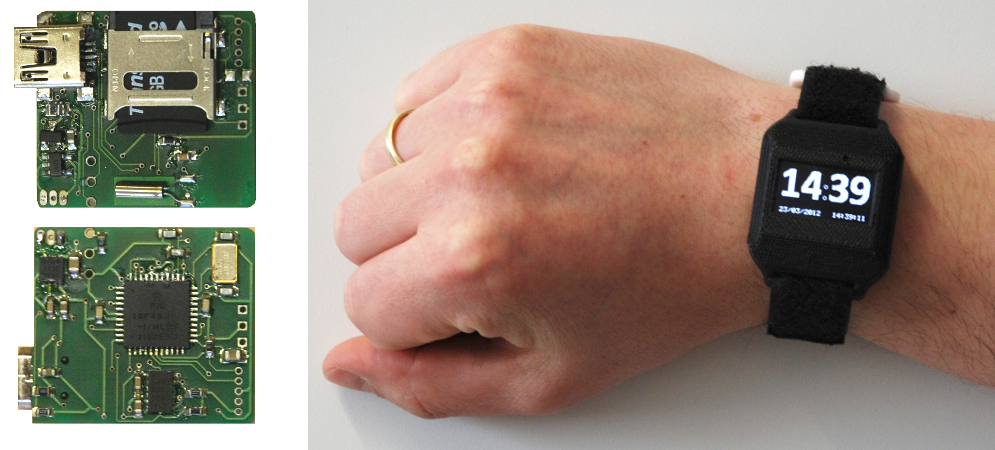
\includegraphics[width=\textwidth]{Images/hardware_sensor.jpg}
	\caption{The inertial data logger featuring a low-power microcontroller, a 3 axis accelerometer, a microSD flash card for storing the sensor data and a USB connector for accessing the stored data (on the left) is being powered by a small lithium polymer battery and is packaged into a plastic case to be worn at the wrist (a version with a OLED display on the right).}
	\label{fig:sensornode}
\end{figure}

The 3D accelerometer sensor is being sampled at $100Hz$, resulting in 10ms equidistant measurements. For efficiency reasons, the sensor data is run-length encoded before being stored locally to the microSD card.

Since the main microcontroller on the sensor node has unoccupied pins, it can be extended with further sensors tailoring different application scenarios. For our scenario, we have added a capacitive proximity sensor, which is described in detail in the next section.


\subsection{Capacitive Proximity Sensor}
power drain: 1mA when active
image : photo
image : board layout and schematics !

The capacitive proximity sensor for the wristband performs measurements in loading mode. The sensing circuit schematic is shown in Figure \ref{}. It is based on a timer that controls the charging and discharging cycles of the virtual capacitor. The timer toggles from charge to discharge at the time when a threshold voltage at the capacitor is reached. This results in an astable operation with succeeding charge/discharge cycles. When the capacitance of the virtual capacitor increases, the charging time will also increase and vice-versa. Therefore, the capacitance is inversely proportional to the number of charging cycles in a given time span. In order to guard the sensor from measuring the capacitance to underlying objects, a shield is placed directly underneath the measuring electrode. The shield is driven with the same potential as the sensing electrode, such that the the capacitance between the two electrodes is neglectable. Using this shielding method, the measured capacitance will only be slightly affected by the grounded underlying arm.

The proximity sensor board generates a clock signal with varying frequency depending on the proximity to body parts, objects and their characteristics. The HedgeHog therefore needs to measure the incoming frequency, which is implemented by counting the signal's edges over the gate time of approximately 9.5ms.

\begin{verbatim}
pseudocode:
  sample the accelerometer sensor
  start frequency counter
  go to sleep for 9.5 ms
  wake-up (timer interrupt)
  stop frequency counter
  read frequency count
\end{verbatim}


\section{Experiment}

This section presents the experimental setup including the activities and the participants, as well as the findings that were obtained during the evaluation.

\subsection{Setup and Scenario}

The experiment setup aims to depict a typical scenario in daily life. Especially in the field of Ambient Assisted Living (AAL), it is desired to monitor activities like drinking, preparing lunch and sleeping. A fine-grained monitoring of such activities may help elderly or people suffering from mental diseases to maintain a healthy day/night rhythm and take action if irregularities occur.

The recorded test set contains the following activities: opening door, sitting on a couch, lying on a couch, grasping into a locker, putting something from a shelf, sitting at the table, preparing a bread with marmalade, eating the bread, pouring water, drinking the water and sleeping. Some of those activities are very hard to recognize without context information, just using wrist-worn accelerometer data. For example, sitting at the table and sitting on a couch are very similar activities. The data of a capacitive proximity sensor can extend this data basis by providing that is related to the material an object is made of.

\begin{figure}
	\centering
		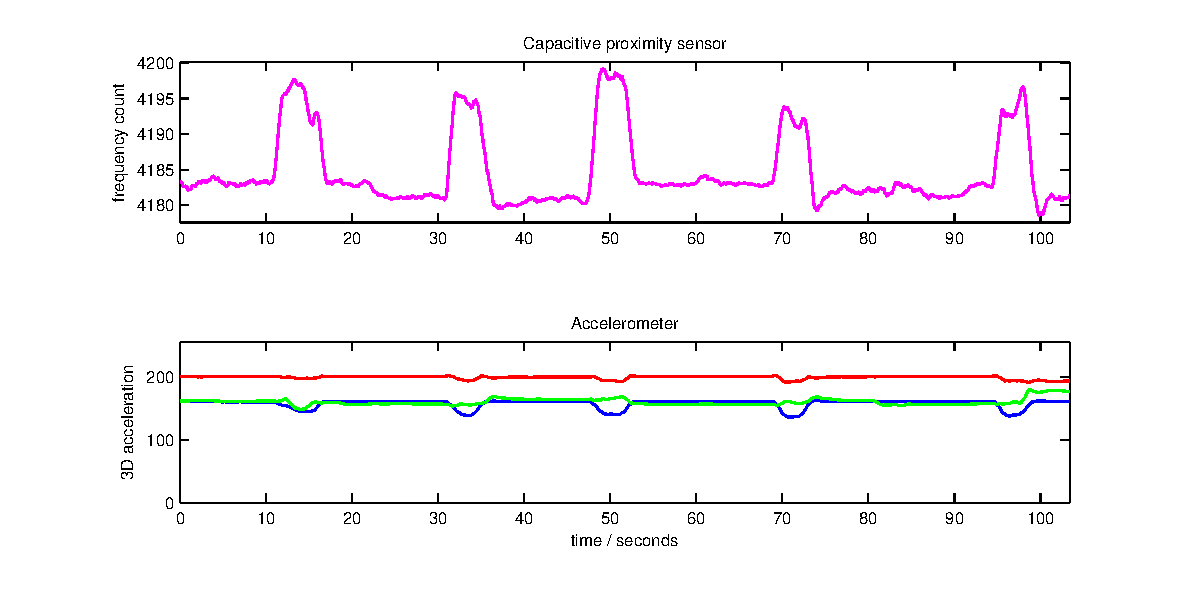
\includegraphics[trim=1.9cm 0.5cm 1.8cm 0.5cm,clip,width=\textwidth]{Images/drinking.pdf}
	\caption{An example of the ``drinking'' activity with raw 3D acceleration data (lower plot) and proximity sensor data (upper plot). The participant took five nips from the glass, while leaving the hands lying on the table in between. These motions can be easily detected in the acceleration as well as proximity data.}
	\label{fig:drinking}
\end{figure}

\begin{figure}
	\centering
		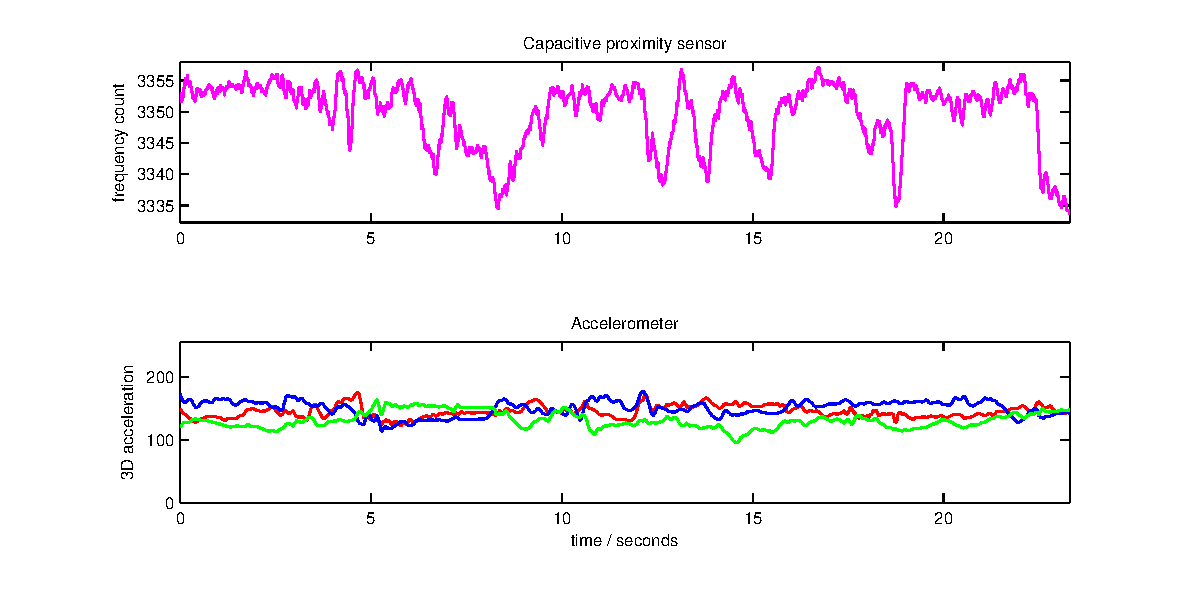
\includegraphics[trim=1.9cm 0.5cm 1.8cm 0.5cm,clip,width=\textwidth]{Images/making-bread.pdf}
	\caption{An example of the ``preparing bread'' activity, where the participants had to put marmalade on a toast. Note, that the acceleration data does not seem to have any characteristic patterns, while the proximity sensor indicates a table, plate, or other objects in ``unmittelbarer n�he''.}
	\label{fig:making-bread}
\end{figure}

[EB: Hier plot von drinking und grasping into locker]

Figure \ref{fig:drinking} depicts the data that was recorded for the activity drinking water. The accelerometer data shows that there periodic up- and down-movements while the capacitive proximity sensor delivers data that is associated to the proximity of the table. Figure \ref{fig:opendoor} illustrates a grasp into a locker while preparing lunch. It is obvious that the locker's bottom surface that is located very closely to the wristband has an influence on the proximity sensor.

In order to evaluate if capacitive proximity sensors in wrist-bands can enhance the performance of activity recognition, we have conducted an evaluation with ten test persons. All test persons received a plot with the activities they were supposed to perform. After manual labeling, we used this test-set as ground truth and performed a cross-validation on an support-vector machine (SVM) classifier once with and once without including the data of the capacitive proximity sensor into the feature set.

[EB MB: kurze Einf�hrung in SVMs]

The classifier was trained with various features that were extracted from windows with the length of 5 seconds. In order to suppress noise contained in the capacitive proximity sensing data, we applied a Gaussian kernel with a size of [TODO] samples. The final feature set contained the arithmetic mean and standard variance of both accelerometer and proximity data. Moreover, we included the median, min and max features for both modalities.

\subsection{Evaluation Results}



\section{Conclusion and Outlook}

\section*{Acknowledgments}
% We would like to thank the students of TU Darmstadt and the employees of Fraunhofer IGD that lent us their sitting and lying abilities for the evaluation. 
We would like to thank our evaluation participants from the TU Darmstadt and the Fraunhofer IGD.

\newpage

\bibliographystyle{splncs03}
\bibliography{references}

\end{document}
